\documentclass[a4paper,12pt]{report}
\usepackage[utf8]{inputenc}


\usepackage{tikz}
\usetikzlibrary{calc}
\usepackage{subcaption}

\begin{document}

\thispagestyle{empty}

\begin{figure}
	\centering
	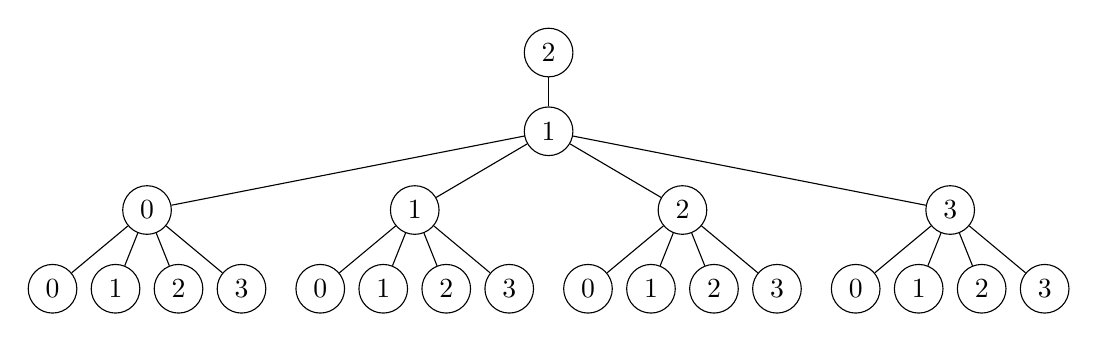
\begin{tikzpicture}
    \node[shape=circle,draw=black] (0) at (0,0) {0};
    \node[shape=circle,draw=black] (1) at (0.8,0) {1};
    %level -1
    \node[shape=circle,draw=black] (16) at (1.2,1) {0};
    %
    \node[shape=circle,draw=black] (2) at (1.6,0) {2};
    \node[shape=circle,draw=black] (3) at (2.4,0) {3};
    
    
    \node[shape=circle,draw=black] (4) at (3.4,0) {0};
    \node[shape=circle,draw=black] (5) at (4.2,0) {1};
    %level -1
    \node[shape=circle,draw=black] (17) at (4.6,1) {1};
    %
    \node[shape=circle,draw=black] (6) at (5,0) {2};
    \node[shape=circle,draw=black] (7) at (5.8,0) {3};
    
    %level -2,-3
    \node[shape=circle,draw=black] (20) at (6.3,2) {1};
    \node[shape=circle,draw=black] (21) at (6.3,3) {2};
    %
    
    \node[shape=circle,draw=black] (8) at (6.8,0) {0};
    \node[shape=circle,draw=black] (9) at (7.6,0) {1};
    %level -1
    \node[shape=circle,draw=black] (18) at (8,1) {2};
    %
    \node[shape=circle,draw=black] (10) at (8.4,0) {2};
    \node[shape=circle,draw=black] (11) at (9.2,0) {3};
    
    
    
    \node[shape=circle,draw=black] (12) at (10.2,0) {0};
    \node[shape=circle,draw=black] (13) at (11,0) {1};
    %level -1
    \node[shape=circle,draw=black] (19) at (11.4,1) {3};
    %
    \node[shape=circle,draw=black] (14) at (11.8,0) {2};
    \node[shape=circle,draw=black] (15) at (12.6,0) {3};

    \path [-] (16) edge node {} (0);
    \path [-] (16) edge node {} (1);
    \path [-] (16) edge node {} (2);
    \path [-] (16) edge node {} (3);
    
    \path [-] (17) edge node {} (4);
    \path [-] (17) edge node {} (5);
    \path [-] (17) edge node {} (6);
    \path [-] (17) edge node {} (7);
    
    \path [-] (18) edge node {} (8);
    \path [-] (18) edge node {} (9);
    \path [-] (18) edge node {} (10);
    \path [-] (18) edge node {} (11);
    
    \path [-] (19) edge node {} (12);
    \path [-] (19) edge node {} (13);
    \path [-] (19) edge node {} (14);
    \path [-] (19) edge node {} (15);
    
    \path [-] (20) edge node {} (16);
    \path [-] (20) edge node {} (17);
    \path [-] (20) edge node {} (18);
    \path [-] (20) edge node {} (19);
    
    \path [-] (21) edge node {} (20);
\end{tikzpicture}
	\caption{Example of one of the best-case scenarios with parameters $K=16$ and $b=4$} \label{tree:3}	
\end{figure}
\end{document}
